\chapter{Machine learning in physics}\label{chap:ml_in_physics}
\thispagestyle{empty}
%%%%%%%%%%%%%%%%%%%%%%%%%%%%%%%%%%%%%%%%%%%%%%%%%%%%%
%   Chapter 2: OUTLINE                              %
%%%%%%%%%%%%%%%%%%%%%%%%%%%%%%%%%%%%%%%%%%%%%%%%%%%%%
Quantum simulation methods like density functional theory and quantum Monte Carlo simulations have facilitated accurate calculations of quantum systems. The amount of quantum simulations performed on a daily basis is immense, but these methods have their restrictions. The time consumption of a DFT simulation increases significantly with the amount of atoms, i.e. $T\sim N^{\alpha}$ with $\alpha \approx 2-3$ and $N$ the number of atoms \citep{KohnNobelLecture}. Thus, if one could predict different material properties more efficiently it would be beneficial to the field of material sciences. The tools of machine learning bring possibilities of doing just that. For example, the situation where a group has done extensive research with quantum simulations on a system of interest. The data achieved by performing these computationally costly simulations can with proper ML methods promote knowledge about the systems of interest as illustrated in \figref{mlandquant}. The figure illustrates how ML can contribute to material sciences by learning from quantum simulated data and additional knowledge about the systems. 
\begin{figure}[ht]
    \centering
    %\iffigure
        \begin{tikzpicture}

        \filldraw[fill=softblue, draw=softblue,ultra thick, rounded corners=15pt, opacity=0.5 ] (-3.5,0.5) rectangle (3.5,2);
        \filldraw[fill=softblue, draw=softblue,ultra thick, rounded corners=15pt, opacity=0.5] (-3.5,-2) rectangle (3.5,-0.5);
        \filldraw[fill=softblue, draw=softblue,ultra thick, rounded corners=15pt, opacity=0.5] (-3.5,-4.5) rectangle (3.5,-3);
        \draw[ultra thick,->, rounded corners=15pt] (3.5,-3.75)--(4.5,-3.75)--(4.5,1.25)--(3.5,1.25);
        \draw[->, ultra thick] (0,0.5)--(0,-0.5);
        \draw[->, ultra thick] (0,-2)--(0,-3);
        
        \node[] at (0,1.25) {Systems of interest (SOI)};
        
        \node[] at (0, -1.25) {Data to be used for ML};
        \node[] at (0,-3.75) {ML model for predictions, $\hat{y}$};
        \node[anchor=south east] at (0,-0.5) {QM computation};
        \node[anchor=south east] at (0,-3) {ML algorithm};
        \node[anchor=west] at (4.5,-1.25) {\rotatebox[origin=c]{270}{Supplementary understanding of SOI}};
    \end{tikzpicture}
    %\fi
    \caption[Machine learning and Quantum Computations]{Illustration of how quantum theory and machine learning can help each other in predicting properties of materials. Machine learning can help speed up the computations by predicting and validating the best candidates as the computation provides raw data for the machine learning model to train on. }
    \label{fig:mlandquant}
\end{figure}
The thoughts about ML and material sciences has consequently brought a lot of attention to the subject and therefore a quick review of the already implemented methods is considered convenient.

\seclab{Implemented ML methods in materials science}{donesofar}

 Several approaches to utilize machine learning algorithms in material science and physics have been made in recent times \citep{mueller_kussesne,criticalrole_descriptor,frameworkforML}. The approaches include predictions of phase diagrams \citep{phasediagram,phase2diagrams}, predictions of various material properties based on data from quantum mechanical computations \citep{rupp,Pilania2013}, interatomic potentials development \citep{hansen2015a,huan2015a, bartok2010a, behler2011a, behler2007a}, predictions of crystal structures  \citep{woodley2008a,madoxx1988,fischer2006a}, discovering and developing density functionals \citep{behler2011ANN}, modelling of crystal lattices \citep{mueller2009a, mueller2012a, seko2009a} along with behavior and processing of complex materials \citep{metzbower2001a, bucholz2012a}.
While some of these are somewhat out of the scope of this project they resemble what can be achieved using machine learning as an asset to established methods in materials science and engineering. An approach related to the procedure of this project was performed by \emph{Rupp et al.} \citep{rupp} who used a ridge regression with a Gaussian Kernel to predict accurate molecular atomization energies. Their data set, which was calculated with\index{Density Functional Theory} (DFT), contained more than 7000 organic molecules, each consisting of up to 7 atoms and they achieved a \emph{Root Mean Squared Error} (RMSE) of $\approx$ 1.3 eV per molecule and a \emph{Mean Absolute Arror} of $\approx$ 0.65 eV per molecule for the machine learning method. 
Another study closely related to this project \citep{criticalrole_descriptor} investigates how to use the Lasso \index{Lasso} method for feature selection in order to predict the difference in energies for two different structures of binary compounds. The purpose of their studies was to outline the critical role of using a suitable feature vector and investigates if a low-dimensional representation of the feature vector would be able to predict the target values. The data set used by \emph{Ghiringhelli} and \emph{Scheffler} consists of 82 binary octet materials, $N=82$, with the target values $\yyy$ = \emph{"The energy differences between the rock salt crystal structure and the zinc blende or wurtzite structures"}. We will strive to do something similar in this project, however, being able to find as low-dimensional feature vectors is unlikely, due our model being more complex as non-octet sets are considered. 
Among all the different ways to implement machine learning in materials science, using the Lasso can serve as a suitable method, since one can create arbitrarily complex feature transformations in accordance to \secref{dataprep} and then penalize the model to reduce complexity to the right amount by using CV for model selection. By doing so, one can introduce the right amount of bias and variance to create a well-generalizing model which keeps its interpretability intact.

\seclab{Predicting the difference in heat of formation between four crystal structures}{main_model}\index{Heat of Formation}\index{Crystal Structures}
%We are living in a time where a lot of research in materials sciences focus on exploration of materials with specific properties for specific purposes. For example, the search for possible materials to be utilized in photovoltaic solar cells. In such a search, it is common to start with a screening phase where a lot of potential candidates are discarded. Even though computer science has evolved a lot in recent years and we can run computationally expensive molecular simulations, methods like DFT and Quantum Clustering can be considered inefficient in such screening processes as they are computationally too costly for the purpose.
The hope of this project is to create a machine learning model able to contribute to the current goals of materials science. Ideally, through the modelling of this project, we can create a universal set of features being able to accurately predict which of the considered crystal structures is the most stable. By doing so, one could reduce the amount of more advanced quantum simulations significantly. 
\subsection{The crystal structures used in the project}
\begin{table}[ht]
    \centering
    \begin{tabular}{cccccc}
    \toprule
    Kind of atom  & \multicolumn{4}{c}{Atom} \\\midrule
    \multirow{11}{*}{\textbf{A}} 
        & Li & Be & B & Na  \\
        & Mg & Al & Si & K  \\
        & Ca & Sc & Ti & Zn \\
        & Ga & Ge & As & Rb  \\ 
        & Sr & Y & Zr & Nb  \\
        & Mo & Ru & Rh & Pd  \\
        & Ag & Cd & In & Sn  \\
        & Sb & Te & Cs & Ba  \\
        & La & Hf & Ta & Re  \\
        & Os & Ir & Pt & Au  \\\midrule
    \multirow{4}{*}{\textbf{B}}    
        & B & C & N & O   \\
        & F & Si & P & S   \\
        & Cl & Ge & As & Se   \\
        & Br & Sb & Te & I   \\\bottomrule
    \end{tabular}
    \caption[The different A and B atoms used]{Identification of the different A and B atoms used to construct the dimers. As seen, there are $44 \times 16 = 704$ different combinations, given us 704 rows of data to be used for machine learning.}
    \label{tab:ABcompounds}
\end{table}

This project has examined four different data sets. Each data set containing the heat of formation, $\Delta H$ of AB compounds calculated with DFT for different crystal structures. The four different structures examined are \emph{Rock Salt} (Rs), \emph{Nickel Arsenide} (NiAs), \emph{Zinc Blende} (Zb) and \emph{Wurtzite} (Wz) and unit cells for each can be seen on \figsref{rs}{nias}{zb}{wz}. In each of the four data sets, there are 44 different A atoms and 16 different B atoms and the data sets contain every combination of A and B. This gives a total of $N = 44 \times 16 = 704$ observations; the different A and B atoms are outlined in \tabref{ABcompounds}.

To get the most data out the model, a machine, that via. a reference structure is able to predict the energy differences between all of the four crystal structures using a multi-target regression, is to prefer. If such a model can be constructed, one would be able get a lot of information out of a a single feature vector $\xxx_i$. 

The target values for the different models that will be constructed is thus, 
\begin{align}
  \hat{y} = \Delta H_{cs \neq r} - \Delta H_{r}  
\end{align}
i.e., if the reference structure as an example is Rock Salt, then $\Delta H_{r} = \Delta H_{\mathrm{Rs}}$ and $\Delta H_{cs \neq r} = \curlyb{\Delta H_{\mathrm{NiAs}},\Delta H_{\mathrm{Zb}},\Delta H_{\mathrm{Wz}}}$
\begin{figure}
    \begin{subfigure}[b]{0.45\textwidth}
    \centering
    \iffigure
    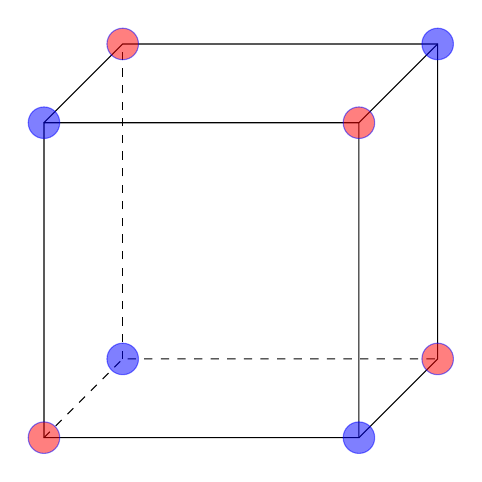
\begin{tikzpicture}
    %Firkant
        \draw[] (0,0) rectangle (4,4)--(5,5);
        \draw[] (0,4)--(1,5)--(5,5)--(5,1)--(4,0);
        \draw[dashed] (0,0)--(1,1)--(5,1) ;
        \draw[dashed] (1,1)--(1,5);

    %Atomer    
        \filldraw[fill=red, draw=blue,opacity=0.5] (0,0) circle (0.2);
        \filldraw[fill=blue, draw=blue,opacity=0.5] (4,0) circle (0.2);
        \filldraw[fill=blue, draw=blue,opacity=0.5] (0,4) circle (0.2);
        \filldraw[fill=red, draw=blue,opacity=0.5] (4,4) circle (0.2);
        \filldraw[fill=blue, draw=blue,opacity=0.5] (1,1) circle (0.2);
        \filldraw[fill=red, draw=blue,opacity=0.5] (5,1) circle (0.2);
        \filldraw[fill=red, draw=blue,opacity=0.5] (1,5) circle (0.2);
        \filldraw[fill=blue, draw=blue,opacity=0.5] (5,5) circle (0.2);
        
        %
    \end{tikzpicture}
    \fi
    \caption{Crystal Structure of Rock Salt (RS). }
    \label{fig:rs}
    \end{subfigure}
    %
    \quad
    %
    \begin{subfigure}[b]{0.45\textwidth}
    \centering
    \iffigure
    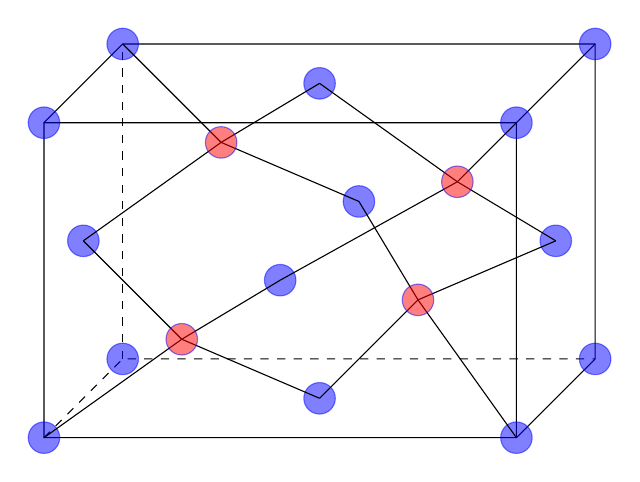
\begin{tikzpicture}
    %Firkant
        \draw[] (0,0) rectangle (6,4)--(7,5);
        \draw[] (0,4)--(1,5)--(7,5)--(7,1)--(6,0);
        \draw[dashed] (0,0)--(1,1)--(7,1) ;
        \draw[dashed] (1,1)--(1,5);

    %Atomer    
        \filldraw[fill=blue, draw=blue,opacity=0.5] (0,0) circle (0.2);
        \filldraw[fill=blue, draw=blue,opacity=0.5] (6,0) circle (0.2);
        \filldraw[fill=blue, draw=blue,opacity=0.5] (0,4) circle (0.2);
        \filldraw[fill=blue, draw=blue,opacity=0.5] (6,4) circle (0.2);
        \filldraw[fill=blue, draw=blue,opacity=0.5] (1,1) circle (0.2);
        \filldraw[fill=blue, draw=blue,opacity=0.5] (7,1) circle (0.2);
        \filldraw[fill=blue, draw=blue,opacity=0.5] (1,5) circle (0.2);
        \filldraw[fill=blue, draw=blue,opacity=0.5] (7,5) circle (0.2);
        %
        \filldraw[fill=blue, draw=blue,opacity=0.5] (0.5,2.5) circle (0.2);
        \filldraw[fill=blue, draw=blue,opacity=0.5] (6.5,2.5) circle (0.2);
        \filldraw[fill=blue, draw=blue,opacity=0.5] (3,2) circle (0.2);
        \filldraw[fill=blue, draw=blue,opacity=0.5] (4,3) circle (0.2);
        \filldraw[fill=blue, draw=blue,opacity=0.5] (3.5,0.5) circle (0.2);
        \filldraw[fill=blue, draw=blue,opacity=0.5] (3.5,4.5) circle (0.2);
        %
        \draw[thin] (0,0)--(1.75,1.25);
        \draw[thin] (0.5,2.5)--(1.75,1.25);
        \draw[thin] (3,2)--(1.75,1.25);
        \draw[thin] (3.5,0.5)--(1.75,1.25);
        
        \draw[thin] (3.5,0.5)--(4.75,1.75);
        \draw[thin] (4,3)--(4.75,1.75);
        \draw[thin] (6,0)--(4.75,1.75);
        \draw[thin] (6.5,2.5)--(4.75,1.75);
        
        \draw[thin] (1,5)--(2.25,3.75);
        \draw[thin] (0.5,2.5)--(2.25,3.75);
        \draw[thin] (3.5,4.5)--(2.25,3.75);
        \draw[thin] (4,3)--(2.25,3.75);
        
        \draw[thin] (3,2)--(5.25,3.25);
        \draw[thin] (3.5,4.5)--(5.25,3.25);
        \draw[thin] (6,4)--(5.25,3.25);
        \draw[thin] (6.5,2.5)--(5.25,3.25);
        %
        \filldraw[fill=red, draw=blue,opacity=0.5] (2.25,3.75) circle (0.2);
        \filldraw[fill=red, draw=blue,opacity=0.5] (1.75,1.25) circle (0.2);
        \filldraw[fill=red, draw=blue,opacity=0.5] (5.25,3.25) circle (0.2);
        \filldraw[fill=red, draw=blue,opacity=0.5] (4.75,1.75) circle (0.2);
    \end{tikzpicture}
    \fi
    \caption{Crystal structure of Zinc blende (ZB).}
    \label{fig:zb}
    \end{subfigure}
    \\
    \begin{subfigure}[b]{0.45\textwidth}
    \centering
    \iffigure
    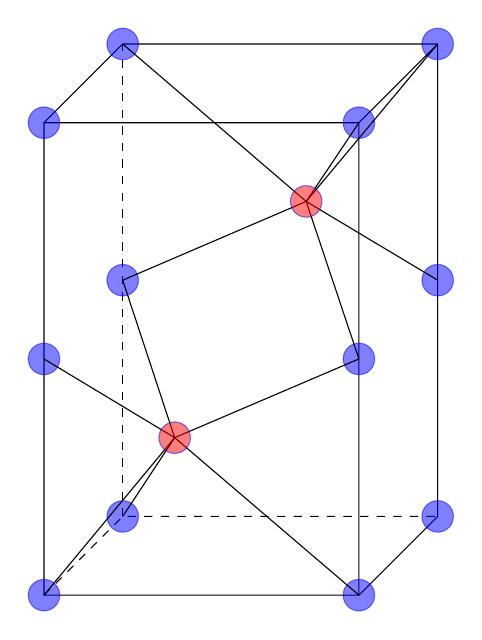
\begin{tikzpicture}
    %Firkant
        \draw[] (0,0) rectangle (4,6)--(5,7);
        \draw[] (0,6)--(1,7)--(5,7)--(5,1)--(4,0);
        \draw[dashed] (0,0)--(1,1)--(5,1) ;
        \draw[dashed] (1,1)--(1,7);
   \iffalse
    %Koordinatsystem
        \draw[thick,->] (-3,0)--(-1,0);
        \draw[thick,->] (-3,0)--(-2.5,0.5);
        \draw[thick,->] (-3,0)--(-3,2);
        \node[anchor=west] at (-1,0) {$x$};
        \node[anchor=west] at (-2.5,0.5) {$y$};
        \node[anchor=west] at (-3,2) {$z$};
    \fi
    %Atomer    
        \filldraw[fill=blue, draw=blue,opacity=0.5] (0,0) circle (0.2);
        \filldraw[fill=blue, draw=blue,opacity=0.5] (4,0) circle (0.2);
        \filldraw[fill=blue, draw=blue,opacity=0.5] (0,3) circle (0.2);
        \filldraw[fill=blue, draw=blue,opacity=0.5] (4,3) circle (0.2);
        \filldraw[fill=blue, draw=blue,opacity=0.5] (1,1) circle (0.2);
        \filldraw[fill=blue, draw=blue,opacity=0.5] (5,1) circle (0.2);
        \filldraw[fill=blue, draw=blue,opacity=0.5] (1,4) circle (0.2);
        \filldraw[fill=blue, draw=blue,opacity=0.5] (5,4) circle (0.2);
        \filldraw[fill=blue, draw=blue,opacity=0.5] (1,7) circle (0.2);
        \filldraw[fill=blue, draw=blue,opacity=0.5] (4,6) circle (0.2);
        \filldraw[fill=blue, draw=blue,opacity=0.5] (5,7) circle (0.2);
        \filldraw[fill=blue, draw=blue,opacity=0.5] (0,6) circle (0.2);
        %
        \draw[thin] (0,0)--(1.66,2);
        \draw[thin] (1,1)--(1.66,2);
        \draw[thin] (0,3)--(1.66,2);
        \draw[thin] (1,4)--(1.66,2);
        \draw[thin] (4,0)--(1.66,2);
        \draw[thin] (4,3)--(1.66,2);
        
        \draw[thin] (4,3)--(3.33,5);
        \draw[thin] (5,4)--(3.33,5);
        \draw[thin] (4,6)--(3.33,5);
        \draw[thin] (5,7)--(3.33,5);
        \draw[thin] (1,7)--(3.33,5);
        \draw[thin] (1,4)--(3.33,5);
        %
        \filldraw[fill=red, draw=blue,opacity=0.5] (3.33,5) circle (0.2);
        \filldraw[fill=red, draw=blue,opacity=0.5] (1.66,2) circle (0.2);
        % 
    \end{tikzpicture}
    \fi
    \caption{Crystal structure of Nickel Arsenide (NiAs)}
    \label{fig:nias}
    \end{subfigure}
    %
    \quad
    %
    \begin{subfigure}[b]{0.45\textwidth}
    \centering
    \iffigure
    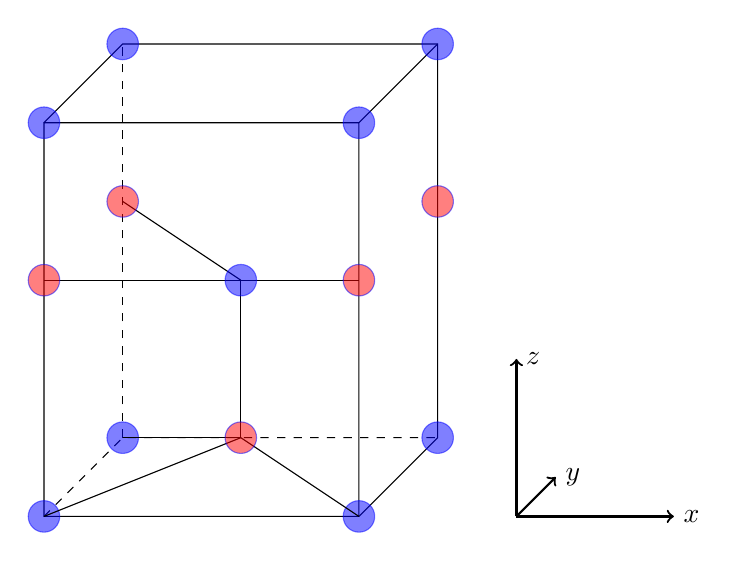
\begin{tikzpicture}
    %Firkant
        \draw[] (0,0) rectangle (4,5)--(5,6);
        \draw[] (0,5)--(1,6)--(5,6)--(5,1)--(4,0);
        \draw[dashed] (0,0)--(1,1)--(5,1) ;
        \draw[dashed] (1,1)--(1,6);

    %Atomer    
        \filldraw[fill=blue, draw=blue,opacity=0.5] (0,0) circle (0.2);
        \filldraw[fill=blue, draw=blue,opacity=0.5] (4,0) circle (0.2);
        \filldraw[fill=blue, draw=blue,opacity=0.5] (0,5) circle (0.2);
        \filldraw[fill=blue, draw=blue,opacity=0.5] (4,5) circle (0.2);
        \filldraw[fill=blue, draw=blue,opacity=0.5] (1,1) circle (0.2);
        \filldraw[fill=blue, draw=blue,opacity=0.5] (5,1) circle (0.2);
        \filldraw[fill=blue, draw=blue,opacity=0.5] (1,6) circle (0.2);
        \filldraw[fill=blue, draw=blue,opacity=0.5] (5,6) circle (0.2);
        %
        \draw[thin] (0,3)--(2.5,3);
        \draw[thin] (1,4)--(2.5,3);
        \draw[thin] (4,3)--(2.5,3);
        
        \draw[thin] (0,0)--(2.5,1);
        \draw[thin] (1,1)--(2.5,1);
        \draw[thin] (4,0)--(2.5,1);
        
        \draw[thin] (2.5,3)--(2.5,1);
        %
        \filldraw[fill=red, draw=blue,opacity=0.5] (0,3) circle (0.2);
        \filldraw[fill=red, draw=blue,opacity=0.5] (1,4) circle (0.2);
        \filldraw[fill=red, draw=blue,opacity=0.5] (4,3) circle (0.2);
        \filldraw[fill=red, draw=blue,opacity=0.5] (5,4) circle (0.2);
        %
        \filldraw[fill=blue, draw=blue,opacity=0.5] (2.5,3) circle (0.2);
        \filldraw[fill=red, draw=blue,opacity=0.5] (2.5,1) circle (0.2);
        
        
      
    %Koordinatsystem
        \draw[thick,->] (6,0)--(8,0);
        \draw[thick,->] (6,0)--(6.5,0.5);
        \draw[thick,->] (6,0)--(6,2);
        \node[anchor=west] at (8,0) {$x$};
        \node[anchor=west] at (6.5,0.5) {$y$};
        \node[anchor=west] at (6,2) {$z$};
    
    \end{tikzpicture}
    \fi
    \caption{Crystal structure of Wurtzite (WZ).}
    \label{fig:wz}
\end{subfigure}

\caption{Unitcells for the four different structures.}
\label{fig:csstruct}
\end{figure}

How the feature vector $\xxx$ for this task has been created, is described in \secref{physicsfeaturevector}.


\subsection{Creating an appropriate feature vector}\label{sec:physicsfeaturevector}
As the desirable feature vector is relatively low-dimensional and our data set containing non-octet compounds is relatively complex, it is very probable that our feature vector should include highly relevant complex attributes. Expert knowledge might come in handy and thus our strategy for creating a suitable feature vector is based on considerations from other people's work, mostly \citep{frameworkforML} and \citep{criticalrole_descriptor}. Initially, a 34-dimensional feature vector is constructed, consisting exclusively of atomic properties of the A- and B atoms and then plenty features will be constructed by feature transformations.

\subsubsection{Atomic attributes}\label{sec:atomic_att}

\pgfplotstableread[col sep=comma] {csv/basic.csv}\basic
\begin{figure}[ht]
    \centering
    \iffigure
    \begin{tikzpicture}
        \begin{axis}[boxplot/draw direction=y,
        xlabel={Attribute}, 
        ylabel={Spread},
        %xtick=data,
        xtick={1,...,17},
        xticklabels={Atom number, Group, Period, Electron negativity, Covalent radius, Atomic radius, Van der Wahls radius, Electron affinity, Ionisation energy, Average oxidation number, Difference in oxidation number, Noble gas, Number of s electrons, Number of p electrons, Number of d electrons, Pettifor radius, Atomization energy pr atom},
        x tick label style={rotate=90,anchor=east},
        enlarge x limits=-1,
        width=1\textwidth,
        height=0.5\textwidth,
        ]
        \foreach \i in {1,...,17} 
            \addplot+[boxplot]
            table[col sep=comma,y index=\i] \basic;
        \end{axis}
    \end{tikzpicture}
    \fi
    \caption[Box-plots for the initial 17 attributes of the A atom]{Boxplot of attributes for the A atom. The data is standardized as described in \secref{statmat}}
    \label{fig:boxplotA}
\end{figure}

\begin{figure}[ht]
    \centering
    \iffigure
    \begin{tikzpicture}
        \begin{axis}[boxplot/draw direction=y,
        xlabel={Attribute}, 
        ylabel={Spread},
        %xtick=data,
        xtick={1,...,17},
        xticklabels={Atom number, Group, Period, Electron negativity, Covalent radius, Atomic radius, Van der Wahls radius, Electron affinity, Ionisation energy, Average oxidation number, Difference in oxidation number, Noble gas, Number of s electrons, Number of p electrons, Number of d electrons, Pettifor radius, Atomization energy pr atom},
        x tick label style={rotate=90,anchor=east},
        enlarge x limits=-1,
        width=1\textwidth,
        height=0.5\textwidth,
        ]
        \foreach \i in {18,...,34} 
            \addplot+[boxplot]
            table[col sep=comma,y index=\i] \basic;
        \end{axis}
    \end{tikzpicture}
    \fi
    \caption[Box-plots for the initial 17 attributes of the B atom]{Boxplot of attributes for the B atom. The data is standardized as described in \secref{statmat}}
    \label{fig:boxplotB}
\end{figure}


\begin{table}[ht]
    \centering
    \begin{tabular}{|p{5cm}|c|l|}\hline
        \textbf{Attribute}                 & \textbf{Unit}  &\textbf{Type}  \\ \hline
        Atom number                 & []    &  Discrete ratio \\ \hline
        Atom group                  & []    &  Discrete ratio \\ \hline
        Atom period                 & []    &  Discrete ratio \\ \hline
        Electron negativity         & [eV]  &  Continuous ratio\\ \hline   
        Covalent radius             & [Å]   &  Continuous ratio \\ \hline
        Atom Radius                 & [Å]   &  Continuous ratio \\ \hline
        Van der Wahls radius        & [Å]   &  Continuous ratio \\ \hline
        Electron affinity           & [eV]  &  Continuous ratio \\ \hline
        Ionisation energy           & [eV]  &  Continuous ratio\\ \hline
        Average oxidation number    & []    &  Continuous ratio\\ \hline 
        Difference between largest and smallest oxidation number & [] & Continuous ratio \\ \hline
        Noble gas number      & []  & Discrete ratio  \\ \hline
        Number of s electrons & []  & Discrete ratio \\ \hline
        Number of p electrons & []  & Discrete ratio \\ \hline
        Number of d electrons & []  & Discrete ratio \\ \hline
        Pettifor radius      & [Å] & Continuous ratio \\ \hline
        Atomization energy per atom  & [eV] & Continuous ratio\\ \hline
    \end{tabular}
    \caption[Overview of the attributes used to describe an atom.]{The 17 attributes loaded from the periodic system used to generate features. The table shows units and attribute types as described in \appref{attribute_types}}
    \label{tab:att}
\end{table}

The atomic attributes in the initial feature vector are outlined in \tabref{att}, but as mentioned in \secref{dataprep}, understanding the data set is crucial. Hence, the following will elaborate on some of the initial attributes. Electron negativity describes the atoms ability to attract another electron, i.e. larger electron negativity means larger attraction. The covalent radius describes the distance an atom would have to another when forming a covalent bond. The atomic radius reflects the ionic radius, which describes the distance to the nearest atom when forming an ionic bond. Another radius to be considered is the Van der Wahls radius. The Van der Wahls radius describes the closest distance one atom can approach another in a hard sphere approximation. Electron affinity describes the cost in energy for adding another electron to the atom in its natural state. The ionization energy is the amount of energy spend to remove the most loosely bounded valence electron. As each atom can have different oxidation numbers the simplest way to describe the amount and size is the average and difference between the largest and smallest. Information about the inner shells of electrons can be found by knowing the noble gasses their atom numbers are listed as an attribute. The outer shells are then described by the number of $s$, $p$ and $d$-electrons in the outer most shell of electrons and the atomization energy is the amount of energy needed to form a mono-atomic gas. Lastly the Pettifor radius is included as an attribute in our feature vector. However, the authors have not been able to find a valid source describing this property. \\

In order to examine the values of the attributes in $\XXXtilde$, two box-plots can be seen in \figtworef{boxplotA}{boxplotB}. In the first figure, \figref{boxplotA}, is shown how the different 17 atomic properties of the A atoms are distributed. Likewise  \figref{boxplotB} has the same visualization purpose for the B atoms. As there are almost three times as many A atoms than B atoms one would expect more variance for the attributes of the A atom, which is the case by comparison of the two figures.\footnote{The observations outside the whiskers occur if they deviate by more than 1.5 $\times$ the interquartile range, measuring from the closest quartile.} It seems like the covalent radius and atomic (or ionic radius) has several observations outside the whiskers for the A atom, while difference in oxidation numbers and number of $p$-electrons each have two. For the B atom the situation is quite different, as there is a single observation outside the whiskers for the Van der Wahls radius, ionisation energy and atomization energy while average oxidation and Pettifor radius each contain two. Overall, the box-plots are in correspondence with what one could expect looking at the list of A and B atoms.


\subsubsection{Feature transformations}\label{sec:featuretrans}\index{Feature Transformations}

As we are ideally trying to predict the difference in heat of formation for the four crystal structures at once, which turns out to be a rather complex task, the initial $M=34$ features might not fit the bill and thus a large number of features are generated from the initial feature vector. As all of the attributes are ratio, the feature transformations can be made arbitrarily complex. 

Most of the initial attributes were loaded with the \texttt{Python}-module \texttt{ELEMENTS} and a few were added from acknowledged databases. The 17 attributes per atom can be seen in \tabref{att} and box-plots for the standardized values\footnote{With respect to the mean and standard deviation of each attribute.} can be found in \figref{boxplotA} and \figref{boxplotB}. The feature vector was then extended by 68 attributes by taking both the natural logarithm and the exponential of each initial attribute, which updated $M=102$ attributes. \\
The idea is to make pairwise linear combinations of different attributes with the same units.\footnote{Energy (eV), Length (Å) and features with no units}
The linear combinations created were:
\begin{itemize}
        \item Sum of pairwise attributes
        \item Absolute value of the difference
        \item The squared sum between 
        \item The difference squared
        \item The exponential values to all of the above.
\end{itemize}
By doing so, we added 288 new features by taking pairwise linear combinations between the \emph{energy} attributes, 168 from the \emph{length} attributes and 1368 from the \emph{no unit} attributes. Therefore, the dimensionality of the feature vector increased to a total of $M=102+288+168+1386=1944$.

The first 102 attributes, i.e. the initial 34 plus the $\log()$ and $\exp()$ to these, were lastly multiplied in every pairwise combination adding $102^2=10404$ features to the 1944 features leaving a $M=12330$ dimensional feature vector ready for modelling.
Hence, since we have $N=704$ AB dimers, the input matrix $\XXX$ contains 704 rows and 12330 columns. \\ In advance of the modelling phase, the data for 32 randomly chosen observations for each crystal structure were put into a secret box with the purpose of final model assessment. We denote this data set, $\mathcal{D}_{\mathrm{test_{box}}}$. The final estimate of relevant erro
 measures is calculated from predictions made on this data set. This leaves us with $N=704-32=672$ observations for training. 

\seclab{The Modelling Phase}{modellingphase}
After creating $\XXX$, one can begin the predictive modelling. As mentioned in \secref{datamodelling}, Lasso will be used exclusively as our modelling method. \\ 
Thus the data matrix $\XXX$, is standardized with respect to the mean and standard deviation of each attribute to construct $\XXXtilde$. If the standard deviation of an attribute is 0, division by the standard deviation of the respective attributes is neglected.

In this section, three different approaches will be examined. In all of these approaches, the heat of formation for the \emph{rock salt} crystal structure was used as reference structure, $\Delta H_{r} = \Delta H_{\mathrm{Rs}}$. Other than having the same reference structure, the different approaches are similar in numerous ways. First and foremost, the models work in an iterative manner. The Lasso is first performed on the 12330 features, where ten different values of the regularization strength $\lambda$\footnote{In the code, the regularization strength is denoted $\alpha$ due to convention by the \texttt{Python} module \texttt{sklearn}} are tested and the optimal model is chosen by cross-validation. Then the generalization error is calculated in accordance to Algorithm \ref{algo:tlcv}, outlined in \chapref{basicConcepts}. Afterwards, relevant measures such as the \emph{average absolute error}, the \emph{maximal absolute error} (\texttt{MaxAE}), and the \emph{root mean squared error} (\texttt{RMSE}), were calculated. Then the features corresponding to the weights which truncated at 0 are discarded and the optimal matrix $\XXX_{\mathrm{opt}}$ is saved to a \texttt{.csv}.\footnote{The optimal matrix for the observations in $\mathcal{D}_{\mathrm{test_{box}}}$ with non-zero weights \texttt{X-opt-test-box} is also saved to a separate \texttt{.csv} file.} The \texttt{attributeNames} corresponding to the non-zero weights are saved to \texttt{.csv} files as well. That was one iteration and every part of the first iteration is then performed again on the new saved matrix, only varying the number of $K$-folds, i.e., $K_1$ and $K_2$ in Algorithm \ref{algo:tlcv}. Four iterations are performed for each of the three models and an example of a code run can be seen in \appref{code}

As the authors of this thesis had very limited machine learning practice before the initialization of this project, a rather simple \emph{single target model} was created as the first approach. 

\subsection{The single-target model}
The \emph{single-target model} tries to predict the difference in heat of formation between the reference structure, \emph{rock salt}, and the remaining three crystal structures one at a time with target values, 
\begin{equation}\label{eq:single_targets}
    y = \Delta H_{cs\neq \mathrm{Rs}} - \Delta H_{\mathrm{Rs}}
\end{equation}
Consequently, the \emph{single-target model} consists of three data sets, $\left\{\mathcal{D}_{\mathrm{NiAs}},\mathcal{D}_{\mathrm{Zb}},\mathcal{D}_{\mathrm{Wz}}\right\}$ with the same initial data matrix $\XXXtilde$ but different target vectors $\left\{\yyy_{\mathrm{NiAs}},\yyy_{\mathrm{Zb}},\yyy_{\mathrm{Wz}}\right\}$. \\ 
In \appref{code}, a code run of an iteration with the \emph{single-target model} is presented.\footnote{The function that imports the data for this model is called \texttt{importdata.py} and be found in the code attachments.} In the \emph{single-target model} the \texttt{LassoCV} method is used in each of the submodels\footnote{One for each crystal structure $\neq$ Rs} for model selection, i.e. finding the optimal regularization strength, and thus find a convenient shrinkage parameter for each crystal structure. Thus, $\XXX_{\mathrm{opt}}$ changes for the different data sets after the first iteration. This might result in better predictive abilities for each submodel, but the targets are less informative compared to the other major models. The results obtained with this model, when tested on the secret box data set, $\mathcal{D}_{\mathrm{test_{box}}}$ will be presented in \chapref{results}. 


\subsection{The multi-target model}
This approach varies from the \emph{single-target model} in several ways. First and foremost, all of the differences in heat of formations between Rs and other crystal structures will be attempted to be predicted simultaneously with a method from \texttt{sklearn} called \texttt{Multi\-Task\-LassoCV}. In this approach, coding wise, the targets corresponding to a single observation are now given as a vector. Hence, the initial data set for this model, $\mathcal{D}_{\mathrm{multi}}$ is now composed of the $N \times M$ input matrix $\XXXtilde$ with a $N \times 3$ target matrix $\underline{\yyy}$,
\begin{equation}
    \underline{\yyy} = \qty[\begin{array}{ccc}
      \yyy_{NiAs}   &   \yyy_{Zb}   &   \yyy_{Wz}  
    \end{array}]
\end{equation}
This method makes the predictions somewhat correlated due to the model only containing a single regularization strength chosen by cross-validation and consequently, one could assume that the prediction accuracy of the model might decrease slightly compared to the \emph{single-target model}. A small problem with this model is the way that it finds non-zero weights. When data is fitted with the \texttt{MultiTaskRegression} method, a weight vector $\bsw$ is assigned to each crystal structure creating a weight matrix, $\boldsymbol{W}$. This weight matrix has a row pr. observation as usual and a column for each target, i.e. $\boldsymbol{W} = \qty[\begin{array}{ccc}
    \bsw_{\mathrm{NiAs}} & \bsw_{\mathrm{Zb}} & \bsw_{\mathrm{Wz}}
\end{array}]$. The problem arises from the fact that as it stands, the zero indices of the weight matrix used to remove unimportant features only evaluates the first column of the weight matrix, i.e. the column corresponding to the NiAs weights. However, even though this might not be the ideal way to remove the unimportant features, the non-zero weights almost exclusively occur for the same features which justifies our choice of action. The results for this model tested on the secret box test set, $\mathcal{D}_{\mathrm{test_{box}}}$ will be presented in \chapref{results} as well.

\subsection{The implicitly informed model}
The final approach, denoted the \emph{implicitly informed model} is quite different from the other models. As the name of the model suggests, the idea is to implicitly inform the model about which difference in heat of formation a target value corresponds to. This is done by creating three extra binary features carrying that information and then create the target vector, $\yyy$ as the intersection between $\left\{\yyy_{\mathrm{NiAs}},\yyy_{\mathrm{Zb}},\yyy_{\mathrm{Wz}}\right\}$, i.e. 
\begin{equation}
    \yyy = \yyy_{\mathrm{NiAs}} \cap \yyy_{\mathrm{Zb}} \cap \yyy_{\mathrm{Wz}}
\end{equation}
Opportunities of this approach include that it increases the number of observations to predict train upon to $N_{\mathrm{total}} = 704 \times 3 = 2112$, where $N_{\mathrm{test}_\mathrm{box}} = 32 \times 3 = 96$, which then leaves us with a total of training observations equal to $N=2112-96=2016$. \\ 
Giving the model implicit information about the crystal structure was done by adding another three binary features to the 102 first features in the feature transformation process described in \secref{featuretrans}. The values of these new binary features will for any feature vector be $\xxx$ is $[1,0,0]$ for a NiAs observation, $[0,1,0]$ for Zb observation and $[0,0,1]$ for Wz. Due to the binary features being added at that time in the feature transformation process, they are included in the rest of feature transformations. Hence, the resulting feature vector of the \emph{implicitly informed model} is $M=13656$ dimensional and $\XXX$ has the form of \eqref{bigX},
\begin{align}
    \boldsymbol{X}&=
    \begin{bmatrix}
        \cdots & 1 &    0   & 0 & \cdots \\
        \cdots & 1 &    0   & 0 & \cdots \\
               &   & \vdots &   & \\
        \cdots & 0 &    1   & 0 & \cdots \\
        \cdots & 0 &    1   & 0 & \cdots \\
               &   & \vdots &   & \\
        \cdots & 0 &    0   & 1 & \cdots \\
        \cdots & 0 &    0   & 1 & \cdots
    \end{bmatrix}\\
    N&=2016\\
    M&=13656
    \label{eq:bigX}
\end{align}
With 96 additional observations reserved for final model assessment (32 for each crystal structure). The hope of this approach is that the machine will find new patterns using the new features and improve performance due to extra training data and knowledge about observations of the other crystal structures. As with the \emph{multi-target model}, a single optimal regularization strength $\lambda$ by CV per iteration is chosen.


\subsection{Comments on the code}\label{sec:codecomment}
The above described methods were implemented in a \texttt{Python} scripts. All of the important scripts for the project can accessed by clicking on the following hyperlink, linking to a \emph{Dropbox} folder: \\
\url{https://www.dropbox.com/sh/pjiq733xi1m61cv/AADRkNQdgWGmHH8kLAb2pYoha?dl=0}











